\chapter{Resultados}\label{cap4_resultados}

{ Após a exposição dos componentes do ambiente de aprendizado e estrutura das
    implementações do processador, é possível realizar análises quantitativas
    e qualitativas dos resultados obtidos.
}

{ As seções desse capítulo explorarão os resultados da síntese e simulação de
    cada versão, além de apresentar resultados de \textit{benchmarks} sintéticos
    a fim de comparar o desempenho de cada implementação e sua viabilidade de uso.
}

{ O código-fonte e demais arquivos da plataforma \textit{RISC-V SiMPLE} denvolvida
    está disponível no \textit{link} \url{https://github.com/LAICO-UnB/riscv-simple}
    com licença \textit{open-source BSD 3-Clause}. O código-fonte e \texttt{.pdf}
    dessa monografia está disponível no \textit{link} \url{https://github.com/arthurbeggs/monografia}
    com licença \textit{open-source BSD 3-Clause}.
}

\section{Síntese dos \textit{soft-cores}}
    { As nove diferentes implementações do processador foram geradas usando o \textit{script}
        \texttt{./make.sh --simulate}, produzindo os arquivos \texttt{.sof} para
        gravação na \textit{FPGA}, os \texttt{.vcd} de simulação em forma de onda
        e os \texttt{.rpt} de resumo do \textit{Quartus}.
    }

    { Os dados da Tabela~\ref{table:synth_resources} foram obtidos dos arquivos
        \texttt{.rpt} e executando os arquivos \texttt{.sof} na placa \textit{DE1-SoC}.
        Cada \textit{ISA} foi carregada com um \textit{benchmark} específico para seu
        conjunto de instruções. Os códigos-fonte podem ser encontrados em
        \texttt{test/assembly\_testbench} e suas versões montadas estão disponíveis
        na pasta \texttt{test/mif\_library}.
    }

    \vspace{0.2cm}
    \begin{longtable}{cc|c|c|c|c|c|c|c|}
        \caption{Características dos sistemas implementados}\label{table:synth_resources}\\
        \cline{3-9}
                                                                &                               & ALMs  & Regs  & Pins  & Mem Bits  & DSPs  & PLLs  & Max Clk   \\
        \cline{2-9}
                                                                & \multicolumn{1}{|c|}{Máximo}  & 32070 & XXXXX & 457   & 4065280   & 87    & 1     & 50MHz     \\
        \hline
        \endfirsthead
        \cline{3-9}
                                                                &                               & ALMs  & Regs  & Pins  & Mem Bits  & DSPs  & PLLs  & Max Clk   \\
        \cline{2-9}
                                                                & \multicolumn{1}{|c|}{Máximo}  & 32070 & XXXXX & 457   & 4065280   & 87    & 1     & 50MHz     \\
        \hline
        \endhead
        \multicolumn{1}{|c}{\multirow{3}{*}{{Uniciclo}}}        & \multicolumn{1}{|c|}{RV32I}   & 4123  & 3160  & 103   & 2805792   & 0     & 1     & 12.5MHz   \\*
        \cline{2-9}
        \multicolumn{1}{|c}{ }                                  & \multicolumn{1}{|c|}{RV32IM}  & 7047  & 3179  & 103   & 2805792   & 12    & 1     & 12.5MHz   \\*
        \cline{2-9}
        \multicolumn{1}{|c}{ }                                  & \multicolumn{1}{|c|}{RV32IMF} & 9411  & 5558  & 103   & 2853408   & 18    & 1     & 3.5MHz    \\
        \hline
        \multicolumn{1}{|c}{\multirow{3}{*}{{Multiciclo}}}      & \multicolumn{1}{|c|}{RV32I}   & 4102  & 3444  & 103   & 2805792   & 0     & 1     & 25MHz     \\*
        \cline{2-9}
        \multicolumn{1}{|c}{ }                                  & \multicolumn{1}{|c|}{RV32IM}  & 6726  & 3471  & 103   & 2805792   & 12    & 1     & 25MHz     \\*
        \cline{2-9}
        \multicolumn{1}{|c}{ }                                  & \multicolumn{1}{|c|}{RV32IMF} & 9108  & 5737  & 103   & 2853408   & 18    & 1     & 25MHz     \\
        \hline
        \multicolumn{1}{|c}{\multirow{3}{*}{\textit{Pipeline}}} & \multicolumn{1}{|c|}{RV32I}   & 4605  & 4139  & 103   & 2805792   & 0     & 1     & 25MHz     \\*
        \cline{2-9}
        \multicolumn{1}{|c}{ }                                  & \multicolumn{1}{|c|}{RV32IM}  & 7376  & 4145  & 103   & 2805792   & 12    & 1     & 25MHz     \\*
        \cline{2-9}
        \multicolumn{1}{|c}{ }                                  & \multicolumn{1}{|c|}{RV32IMF} & 9750  & 6568  & 103   & 2853408   & 18    & 1     & 25MHz*    \\
        \hline
    \end{longtable}

    { Ao analisar a tabela, podemos tirar as seguintes conclusões: }
    \begin{itemize}
        \item   O número de \textit{PLLs} e de pinos não muda entre as implementações,
            pois somente um \textit{PLL} é utilizado para gerar os sinais de relógio da
            \textit{FPGA}, e o \textit{pinout} do módulo \textit{top level} não é alterado
            entre as versões do processador. Variação nesses valores representaria um erro;
        \item   O número de \textit{DSPs} é \texttt{0} para a \textit{ISA} \textit{RV32I},
            \texttt{12} para a \textit{RV32IM} e \texttt{18} para a \textit{RV32IMF}. Os
            \textit{DSPs} apenas são utilizados nas operações de \textit{mul/div} e ponto flutuante;
        \item   A quantia de \textit{bits} de memória utilizados permanece igual para
            todas as implementações das \textit{ISAs} \textit{RV32I} e \textit{RV32IM}.
            Todas as implementações da \textit{RV32IMF} também utilizam a mesma quantia de
            \textit{bits}, que é levemente maior que nas outras duas arquiteturas;
        \item   Como é de se esperar, a quantia de \textit{ALMs} e \textit{registradores}
            aumenta ao implementar mais extensões numa mesma microarquitetura;
        \item   A microarquitetura multiciclo utiliza a menor quantia de recursos entre
            as três, resultado esperado já que sua implementação reutiliza estruturas como
            a ULA na sua execução por microcódigo, enquanto as outras arquiteturas utilizam
            mais de um somador com funções específicas em seu \textit{datapath};
        \item   A frequência máxima de operação do multiciclo se manteve constante para as
            três \textit{ISAs} implementadas e teve bom desempenho;
        \item   A frequência de operação do uniciclo foi a mais baixa entre os sistemas
            implementados, como era esperado. Com o uso de operações de ponto flutuante,
            sua frequência máxima foi bastante penalizada;
        \item   A implementação da \textit{ISA RV32IMF} no \textit{pipeline} apresenta
            erros devido a \textit{forwards e hazards} não tratados ou tratados de maneira
            incorreta. Para as extensões \textit{I} e \textit{IM} sua frequência máxima
            é de 25MHz, como no multiciclo. A extensão \textit{IMF} apresenta erros durante
            sua execução, então não é possível confirmar que sua frequência máxima também é
            de 25MHz.
    \end{itemize}

\section{Formas de Onda das Simulações}
    { As Figuras \ref{fig:gtkwave_uni}, \ref{fig:gtkwave_multi} e \ref{fig:gtkwave_pipe}
        mostram as visualizações criadas para as simulações dos \textit{soft-cores}
        \textit{RV32IMF} uniciclo, multiciclo e \textit{pipeline} respectivamente.
        Nelas, as instruções passam por um \textit{desassembler}, os registradores
        são mostrados com seus nomes mnemônicos e os sinais possuem cores diferentes
        dependendo de sua origem.
    }

    { Com essas visualizações, o processo de depuração do processador é facilitado.
        Alguns \textit{bugs} do \textit{pipeline} só puderam ser identificados graças
        à simulação. Os sinais adicionados são suficientes para a maioria das inspeções,
        mas se necessário, novos sinais podem ser adicionados.
    }

    \begin{figure}[H]
    \centering
        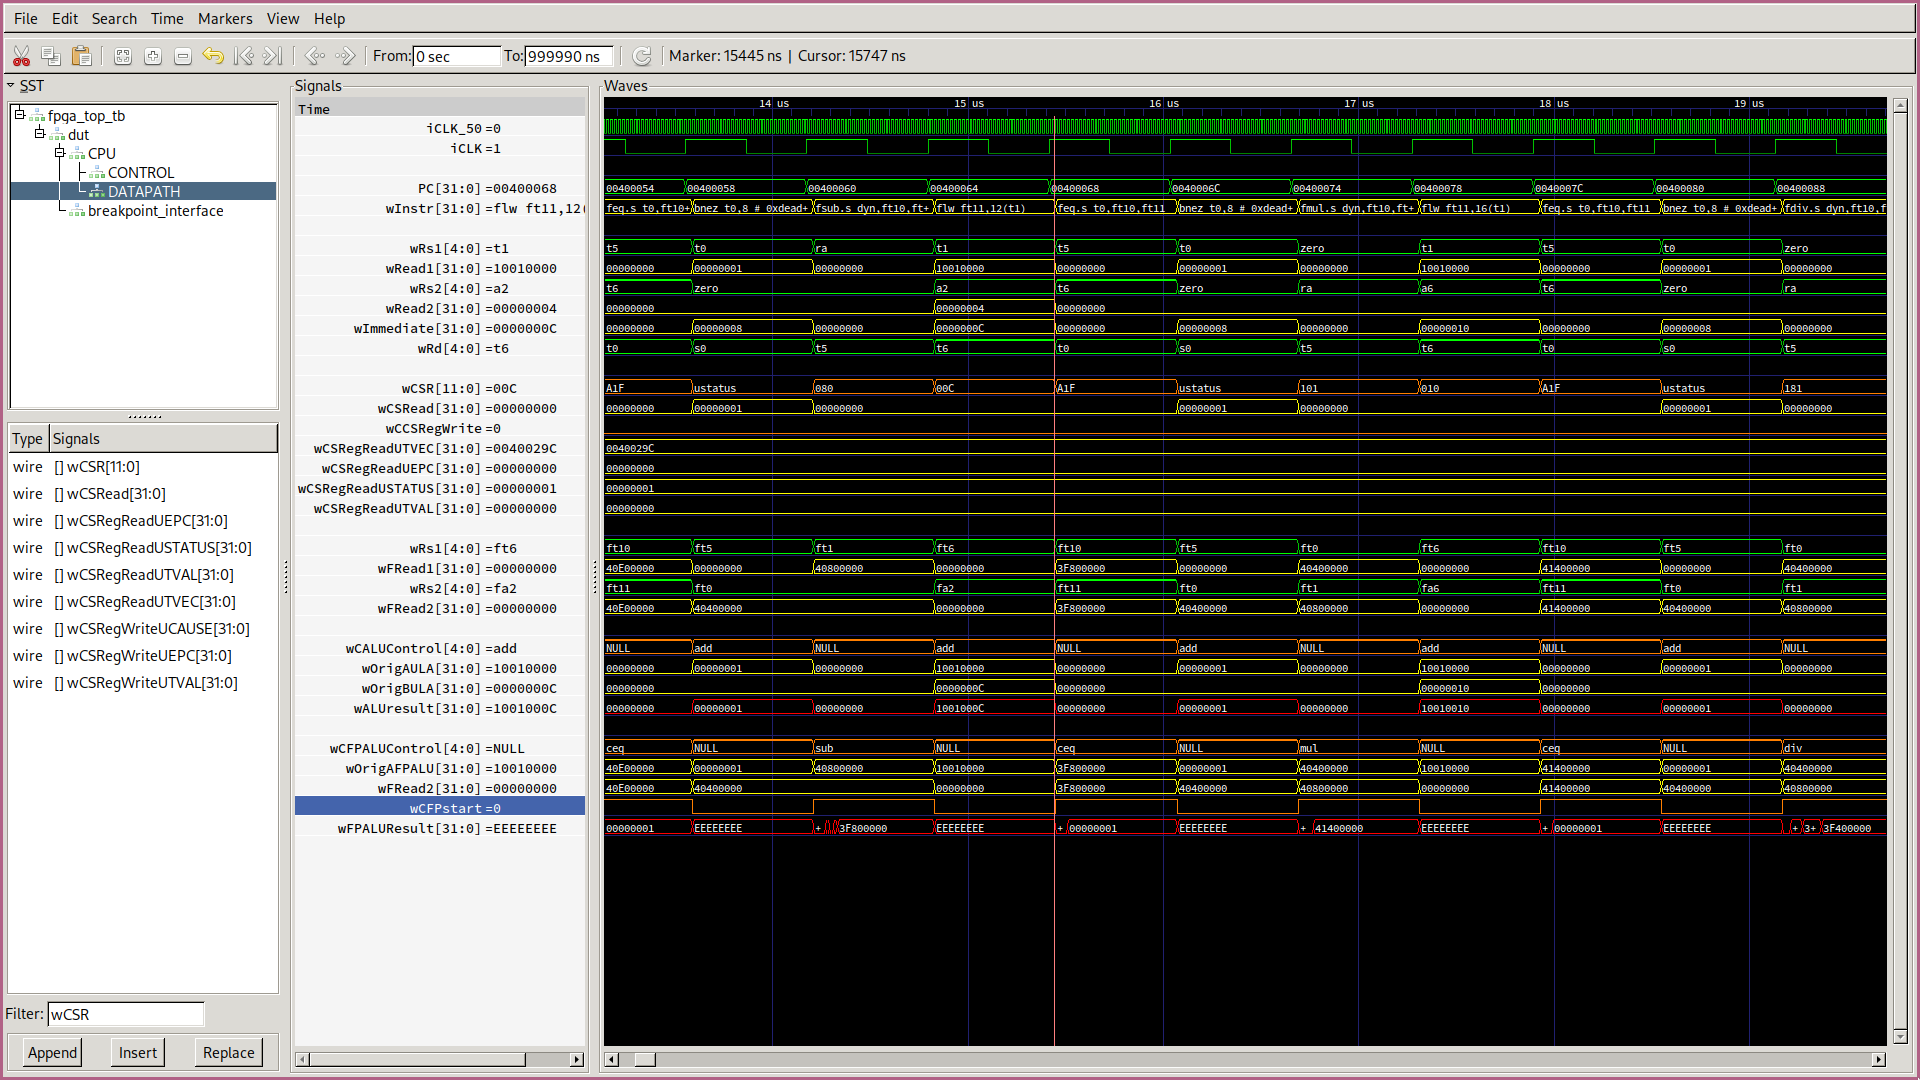
\includegraphics[width=0.9\linewidth]{../images/gtkwave/gtkwave_uni.png}
        \caption{Visualização das formas de onda \textit{soft-core} \textit{RV32IMF} uniciclo}
        \label{fig:gtkwave_uni}
    \end{figure}

    \begin{figure}[H]
    \centering
        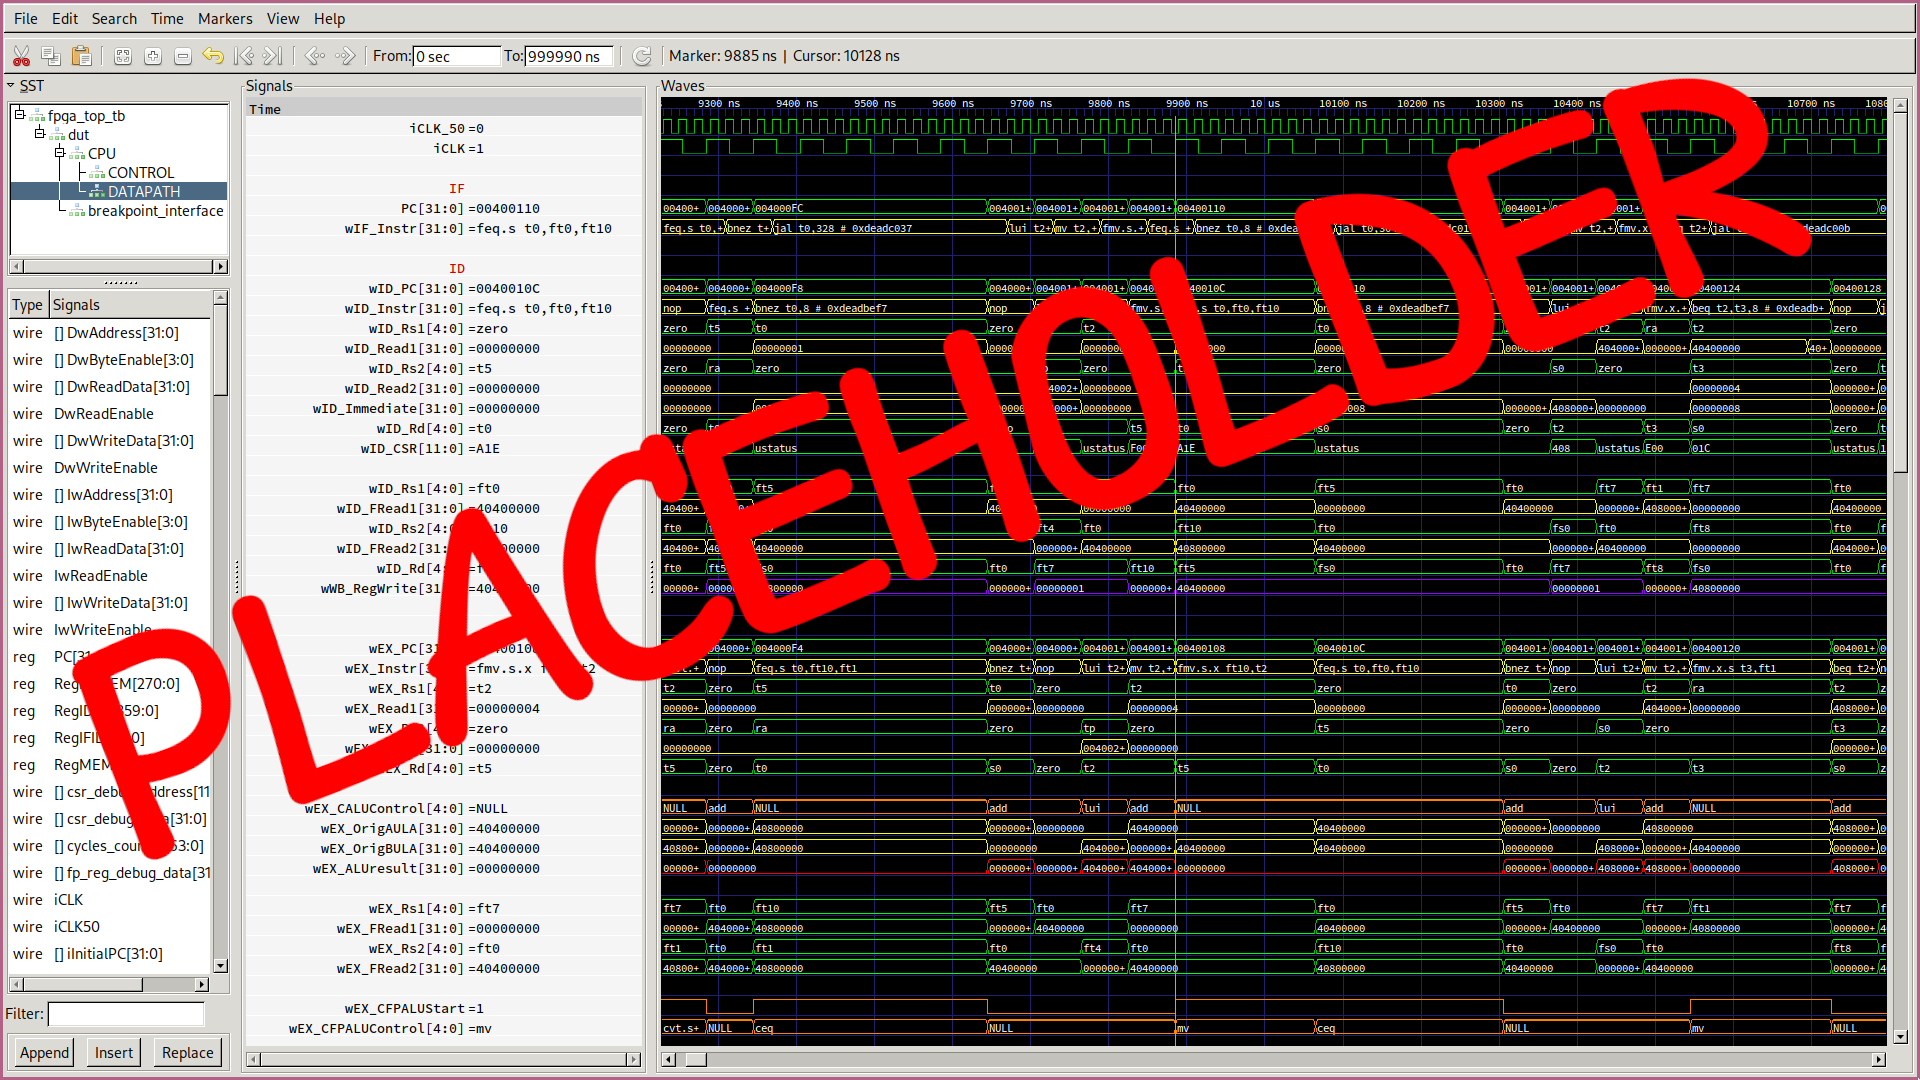
\includegraphics[width=0.9\linewidth]{../images/gtkwave/gtkwave_multi.png}
        \caption{Visualização das formas de onda \textit{soft-core} \textit{RV32IMF} multiciclo}
        \label{fig:gtkwave_multi}
    \end{figure}

    \begin{figure}[h]
    \centering
        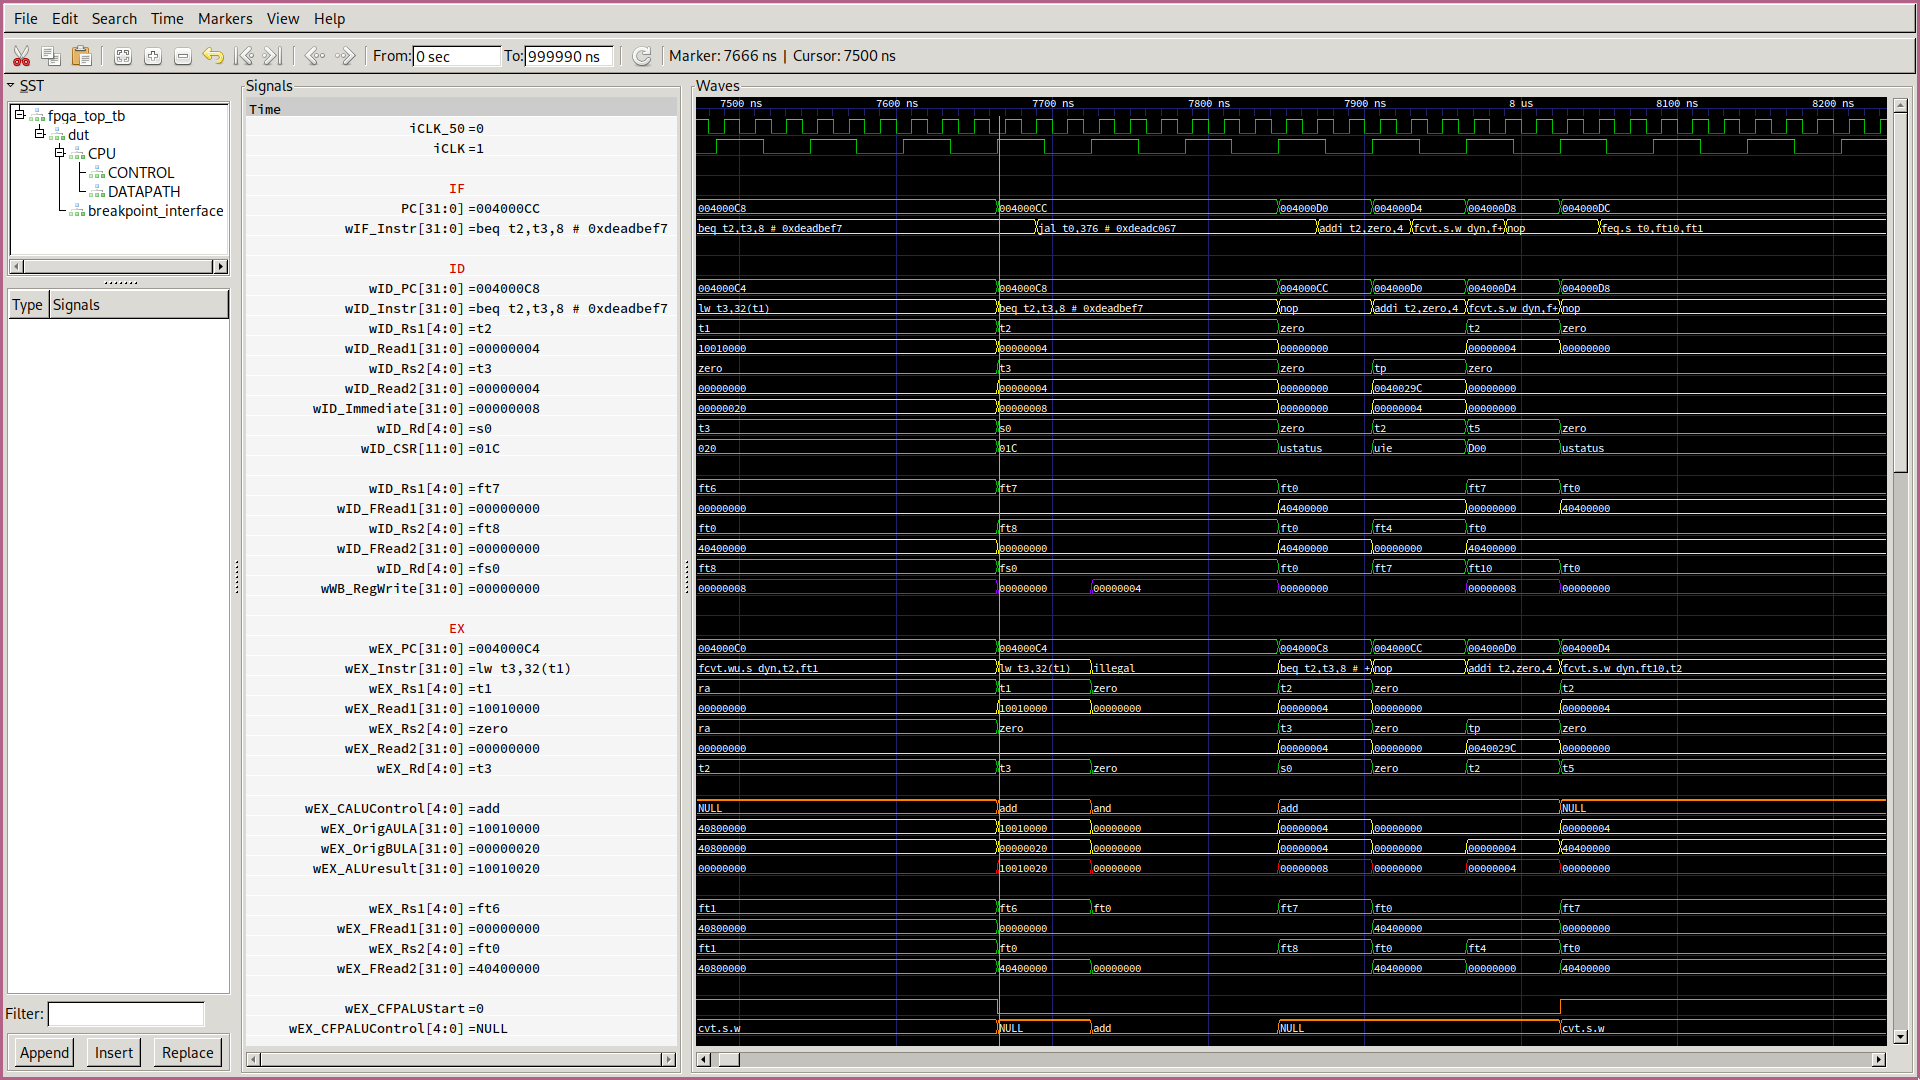
\includegraphics[width=0.9\linewidth]{../images/gtkwave/gtkwave_pipe.png}
        \caption{visualização das formas de onda \textit{soft-core} \textit{rv32imf} \textit{pipeline}}
        \label{fig:gtkwave_pipe}
    \end{figure}

    { Na Figura~\ref{fig:gtkwave_zoom}, a visualização da forma de onda do
        multiciclo é ampliada para mostrar os detalhes do sinal \texttt{IR}
        mostrando o assembly da instrução em vez do seu valor em hexadecimal.
        Também mostra os seletores de registradores \texttt{wRs1} e \texttt{wRS2}
        exibindo o mnemônico dos registradores. Os demais sinais permitem entender
        o funcionamento interno do processador e identificar erros de lógica.
    }

    \begin{figure}[h]
    \centering
        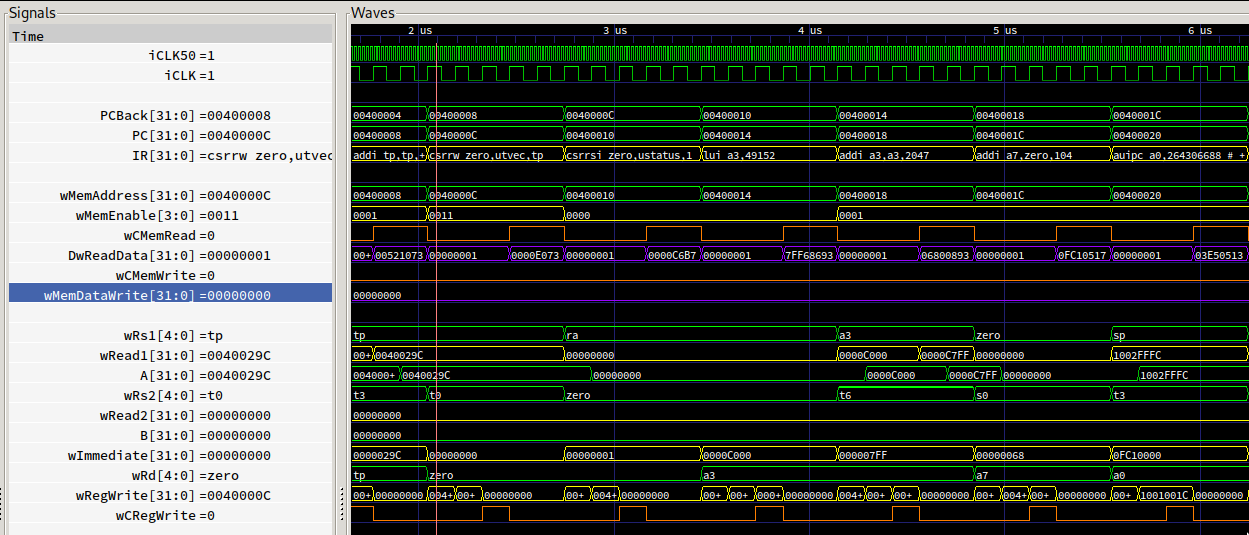
\includegraphics[width=1\linewidth]{../images/gtkwave/gtkwave_zoom.png}
        \caption{\textit{Zoom} da visualização das formas de onda do multiciclo \textit{RV32IMF}}
        \label{fig:gtkwave_zoom}
    \end{figure}

\clearpage
\section{\textit{Benchmarks}}
    { Para analisar o desempenho das diferentes implementações, três \textit{benchmarks}
        foram realizados. Cada um dos \textit{benchmarks} foi criado para rodar
        em uma \textit{ISA} específica. Assim, temos um teste para a arquitetura
        \textit{RV32I}, um segundo para a \textit{RV32IM} e por último, um para a
        \textit{RV32IMF}. Pela escassez de instruções implementadas por \textit{software}
        caso uma extensão não esteja disponível, fazer um único arquivo de teste
        e executá-lo nas 9 implmementações não é ideal.
    }

    { Os três \textit{benchmarks} realizam 1000 ciclos de operações específicas de sua
        extensão. O valor do registrador de estado \texttt{time} será usado para verificar
        quantos milissegundos foram necessários para completar o teste.  Essa análise tem
        como objetivo comparar o desempenho das diferentes microarquiteturas para o mesmo
        \textit{workload} dispondo do mesmo conjunto de instruções. Os testes são executados
        utilizando a frequência máxima da implementação, conforme a
        Tabela~\ref{table:synth_resources} e seus códigos-fonte se encontram
        em \texttt{test/assembly\_testbench}.
    }

    \begin{longtable}{cc|c|c|c|}
        \caption{Comparativo de desempenho de cada \textit{ISA} em microarquiteturas distintas}\label{table:benchmark}\\
        \cline{3-5}
                                                                &                               & RV32I       & RV32IM      & RV32IMF   \\
        \hline
        \endfirsthead
        \endhead
        \multicolumn{1}{|c}{\multirow{2}{*}{{Uniciclo}}}        & \multicolumn{1}{|c|}{time}    & 30 ms       & 18 ms       & 52 ms \\
        \cline{2-5}
        \multicolumn{1}{|c}{ }                                  & \multicolumn{1}{|c|}{clock}   & 12.5MHz     & 12.5MHz     & 3.5MHz \\
        \hline
        \multicolumn{1}{|c}{\multirow{2}{*}{{Multiciclo}}}      & \multicolumn{1}{|c|}{time}    & 72 ms       & 46 ms       & 61 ms \\
        \cline{2-5}
        \multicolumn{1}{|c}{ }                                  & \multicolumn{1}{|c|}{clock}   & 25MHz       & 25MHz       & 25MHz \\
        \hline
        \multicolumn{1}{|c}{\multirow{2}{*}{\textit{Pipeline}}} & \multicolumn{1}{|c|}{time}    & 21 ms       & 16 ms       & erro \\
        \cline{2-5}
        \multicolumn{1}{|c}{ }                                  & \multicolumn{1}{|c|}{clock}   & 25MHz       & 25MHz       & 25MHz \\
        \hline
    \end{longtable}

    { Pelos resultados obtidos, é possível ver que, apesar do multiciclo ter
        frequência mais alta que o uniciclo, em todas as implementações ele demorou
        mais a completar os testes. Para as \textit{ISAs RV32I} e \textit{RV32IM},
        o \textit{pipeline} foi a versão mais rápida. Na \textit{ISA RV32IMF},
        existem erros na execução do \textit{pipeline}, e por isso não foi possível
        compará-la com as demais.
    }

\section{Observações Finais dos Resultados}
    { Vimos no capítulo o resultado da execução de pequenos testes da plataforma
        desenvolvida, tanto em simulação por forma de onda quanto na execução de
        \textit{benchmarks} na \textit{FPGA DE1-SoC}. Das nove implementações,
        uma apresenta falhas a tempo de execução, a \textit{RV32IMF} em
        \textit{pipeline} de cinco estágios. No entanto, a configuração feita para
        a ferramenta de simulação de forma de onda trará mais um instrumento para
        encontrar e solucionar o defeito de código.
    }

    { O próximo capítulo encerrará o presente trabalho fazendo observações
        pertinentes aos resultados obtidos, à viabilidade do uso da plataforma
        desenvolvida para os propósitos desejados e perspectivas futuras,
        tratando de possíveis melhorias e expansão do escopo.
    }

